\chapter*{Summary}
\addcontentsline{toc}{chapter}{Summary}
Major Project Phase 2 builds ScamGuard, a system that reads one SMS or other message, decides whether it is a scam or genuine, explains the decision and suggests the next step. The completed work includes the ScamGuard-IN-2026 dataset of 11,399 messages with an audit of its labels, campaign-aware splitting with MinHash, the TF-IDF and logistic-regression detector joined with 31 intent patterns, the FastAPI back end with its PostgreSQL database, the Next.js web application in English and Hindi, and the cross-domain generalization and adaptation study proposed by our guide. On 1,874 real messages from campaigns the model never saw, the deployed system scores 97.1\% accuracy with 3.2\% false alarms. In the cross-domain study, adding 10\% of a labelled Indian pool (143 messages) raised the mean Indian F1 of Logistic Regression from 0.681 to 0.964. These are results on public datasets that we audited ourselves; they do not claim the same accuracy on all future scam messages.

Key deliverables achieved include:

\textbf{Dataset and Label Audit:} ScamGuard-IN-2026 was assembled from public reports, real Indian SMS, advisory texts and synthetic training messages. An audit of 2,922 decisions showed that 19.5\% of the retained reports were genuine, and the corrected labels cut false alarms from 34.0\% to 2.6\% for the classifier alone.

\textbf{Detection Engine:} The classifier uses 35,148 word and character TF-IDF features, and the intent evidence and ten protective signals are fused with a capped adjustment so that each verdict can be explained in plain words.

\textbf{Cross-Domain Study:} Two models trained on the UCI SMS Spam Collection were tested unchanged on an Indian SMS dataset. Three seeds and McNemar's test (all 36 comparisons significant at $p<0.05$) show that a small amount of local data repairs most of the drop.

\textbf{Application and Deployment:} The Next.js front end runs on Vercel, the FastAPI back end on Render and the database on Neon, with 836 back-end and 14 front-end automated tests, a cross-domain page and a Streamlit demo.
\clearpage
\renewcommand{\bibname}{References}
\addcontentsline{toc}{chapter}{References}
\addcontentsline{toc}{chapter}{Appendix A: Bibliography}
\begin{thebibliography}{99}\small
\bibitem{agarwal2025fishing} S. Agarwal, A. Papasavva, G. Suarez-Tangil, and M. Vasek, ``Fishing for smishing: Understanding SMS phishing infrastructure and strategies by mining public user reports,'' in \textit{Proc. ACM Internet Measurement Conference (IMC '25)}, Madison, WI, USA, 2025, doi: 10.1145/3730567.3764431.
\bibitem{agarwal2026overview} S. Agarwal, G. Suarez-Tangil, and M. Vasek, ``An overview of 7726 user reports: Uncovering SMS scams and scammer strategies,'' in \textit{Proc. Network and Distributed System Security Symposium (NDSS)}, San Diego, CA, USA, 2026.
\bibitem{pritom2026sms} M. M. A. Pritom, S. M. Sanjari, M. Mia, A. M. Shibli, S. M. M. Hossain, M. Ismail, and S. Xu, ``Short message service (SMS) phishing attacks and defenses: A systematic review,'' arXiv:2604.11429, 2026.
\bibitem{almeida2011contributions} T. A. Almeida, J. M. G\'omez Hidalgo, and A. Yamakami, ``Contributions to the study of SMS spam filtering: New collection and results,'' in \textit{Proc. 11th ACM Symposium on Document Engineering}, Mountain View, CA, USA, 2011, pp. 259--262.
\bibitem{almeida2013towards} T. A. Almeida, J. M. G\'omez Hidalgo, and T. P. Silva, ``Towards SMS spam filtering: Results under a new dataset,'' \textit{International Journal of Information Security Science}, vol. 2, no. 1, pp. 1--18, 2013.
\bibitem{roy2020deep} P. K. Roy, J. P. Singh, and S. Banerjee, ``Deep learning to filter SMS spam,'' \textit{Future Generation Computer Systems}, vol. 102, pp. 524--533, 2020.
\bibitem{mishra2020smishing} S. Mishra and D. Soni, ``Smishing Detector: A security model to detect smishing through SMS content analysis and URL behavior analysis,'' \textit{Future Generation Computer Systems}, 2020.
\bibitem{sonowal2018smidca} G. Sonowal and K. S. Kuppusamy, ``SmiDCA: An anti-smishing model with machine learning approach,'' \textit{The Computer Journal}, vol. 61, no. 8, pp. 1143--1157, 2018, doi: 10.1093/comjnl/bxy039.
\bibitem{goel2024ml} D. Goel, H. Ahmad, A. K. Jain, and N. K. Goel, ``Machine learning driven smishing detection framework for mobile security,'' arXiv:2412.09641, 2024.
\bibitem{timko2024smishing} D. Timko and M. L. Rahman, ``Smishing Dataset I: Phishing SMS dataset from Smishtank.com,'' in \textit{Proc. 14th ACM Conference on Data and Application Security and Privacy (CODASPY '24)}, Porto, Portugal, 2024, doi: 10.1145/3626232.3653282.
\bibitem{ali2025moz} F. D. M. A. Ali, S. M. Saide, R. Sousa-Silva, and H. Lopes Cardoso, ``MOZ-Smishing: A benchmark dataset for detecting mobile money frauds,'' in \textit{Proc. 6th Workshop on African Natural Language Processing}, Vienna, Austria, 2025, pp. 158--166, doi: 10.18653/v1/2025.africanlp-1.23.
\bibitem{labonne2023spamt5} M. Labonne and S. Moran, ``Spam-T5: Benchmarking large language models for few-shot email spam detection,'' arXiv:2304.01238, 2023.
\bibitem{ahmadi2025llm} M. Ahmadi, M. Khajavi, A. Varmaghani, A. Ala, K. Danesh, and D. Javaheri, ``Leveraging large language models for cybersecurity: Enhancing SMS spam detection with robust and context-aware text classification,'' arXiv:2502.11014, 2025.
\bibitem{northcutt2021confident} C. Northcutt, L. Jiang, and I. Chuang, ``Confident learning: Estimating uncertainty in dataset labels,'' \textit{Journal of Artificial Intelligence Research}, vol. 70, pp. 1373--1411, 2021, doi: 10.1613/jair.1.12125.
\bibitem{lee2022dedup} K. Lee, D. Ippolito, A. Nystrom, C. Zhang, D. Eck, C. Callison-Burch, and N. Carlini, ``Deduplicating training data makes language models better,'' in \textit{Proc. 60th Annual Meeting of the ACL}, Dublin, Ireland, 2022, pp. 8424--8445, doi: 10.18653/v1/2022.acl-long.577.
\bibitem{kapoor2023leakage} S. Kapoor and A. Narayanan, ``Leakage and the reproducibility crisis in machine-learning-based science,'' \textit{Patterns}, 2023, doi: 10.1016/j.patter.2023.100804.
\bibitem{broder1997resemblance} A. Z. Broder, ``On the resemblance and containment of documents,'' in \textit{Proc. Compression and Complexity of SEQUENCES 1997}, Positano, Italy, 1997, doi: 10.1109/SEQUEN.1997.666900.
\bibitem{salton1988term} G. Salton and C. Buckley, ``Term-weighting approaches in automatic text retrieval,'' \textit{Information Processing \& Management}, vol. 24, no. 5, pp. 513--523, 1988, doi: 10.1016/0306-4573(88)90021-0.
\bibitem{pedregosa2011scikit} F. Pedregosa \textit{et al.}, ``Scikit-learn: Machine learning in Python,'' \textit{Journal of Machine Learning Research}, vol. 12, pp. 2825--2830, 2011.
\bibitem{indiasms2024} JuniorAlive, ``India Spam SMS Classification,'' GitHub repository, 2024. [Online]. Available: https://github.com/junioralive/india-spam-sms-classification
\bibitem{bendavid2010theory} S. Ben-David, J. Blitzer, K. Crammer, A. Kulesza, F. Pereira, and J. W. Vaughan, ``A theory of learning from different domains,'' \textit{Machine Learning}, vol. 79, pp. 151--175, 2010, doi: 10.1007/s10994-009-5152-4.
\bibitem{pan2010survey} S. J. Pan and Q. Yang, ``A survey on transfer learning,'' \textit{IEEE Transactions on Knowledge and Data Engineering}, vol. 22, no. 10, pp. 1345--1359, 2010, doi: 10.1109/TKDE.2009.191.
\bibitem{daume2007frustratingly} H. Daum\'e III, ``Frustratingly easy domain adaptation,'' in \textit{Proc. 45th Annual Meeting of the Association for Computational Linguistics}, Prague, Czech Republic, 2007, pp. 256--263.
\bibitem{mcnemar1947note} Q. McNemar, ``Note on the sampling error of the difference between correlated proportions or percentages,'' \textit{Psychometrika}, vol. 12, no. 2, pp. 153--157, 1947, doi: 10.1007/BF02295996.
\bibitem{dietterich1998approximate} T. G. Dietterich, ``Approximate statistical tests for comparing supervised classification learning algorithms,'' \textit{Neural Computation}, vol. 10, no. 7, pp. 1895--1923, 1998, doi: 10.1162/089976698300017197.
\end{thebibliography}
\clearpage
\chapter*{SDG Analysis}
\addcontentsline{toc}{chapter}{Appendix B: POs and PSOs Mapped}
The ScamGuard project aligns with the following United Nations Sustainable Development Goals (SDGs):

\textbf{SDG 16: Peace, Justice and Strong Institutions (target 16.4, illicit financial flows).} Many payment frauds begin with one text message. If a user spots the trap before paying or sharing an OTP, the money never reaches the fraudster. The application also sends users to the official channels: the 1930 helpline and cybercrime.gov.in.

\textbf{SDG 8: Decent Work and Economic Growth (target 8.10, access to financial services).} People adopt digital payments only when they feel safe using them. Telling real bank and UPI alerts from imitations helps keep that confidence.

\textbf{SDG 9: Industry, Innovation and Infrastructure (target 9.c, access to ICT).} The model is small, runs on free cloud servers and replies in milliseconds, so the service costs its users nothing. The cross-domain results add that a model can be moved to a new region with a few hundred labelled local messages.

\textbf{SDG 10: Reduced Inequalities.} Hindi support and a simpler elder mode are meant for the people fraudsters target most and English-only tools serve least.

\vspace{0.5cm}
{\small
\renewcommand{\arraystretch}{1.2}
\setlength{\tabcolsep}{6pt}
\begin{longtable}{|L{3.6cm}|c|L{7.2cm}|}
\caption*{Table 2: Programme Outcomes Mapping with ScamGuard and Domain Adaptation}\\
\hline
\textbf{PROGRAMME OUTCOMES} & \textbf{Level (1/2/3)} & \textbf{Justification if addressed} \\
\hline
\endfirsthead
\hline
\textbf{PROGRAMME OUTCOMES} & \textbf{Level (1/2/3)} & \textbf{Justification if addressed} \\
\hline
\endhead
PO1 & 3 & Machine learning, NLP and statistics are used both to build the scam classifier and to judge how well it works. \\
\hline
PO2 & 3 & We studied why current filters struggle with Indian SMS and traced the problem to unchecked labels, leaky evaluation and domain shift. \\
\hline
PO3 & 3 & A dataset, a detector and a web application were designed to meet targets for accuracy, speed and explanation. \\
\hline
PO4 & 3 & Experiments are controlled: held-out campaigns, a separate target domain, bootstrap intervals, three seeds and significance tests. \\
\hline
PO5 & 3 & Modern tools throughout: scikit-learn, MinHash, FastAPI, Next.js, Streamlit, GitHub Actions and cloud hosting. \\
\hline
PO6 & 3 & Helps people avoid financial fraud and directs them to the official places to report it. \\
\hline
PO7 & 1 & Light enough for free, low-power servers; no GPU is needed. \\
\hline
PO8 & 3 & Personal data is masked, dataset licences are followed and the limitations are stated openly. \\
\hline
PO9 & 3 & Four students shared the work on data, model, back end and front end. \\
\hline
PO10 & 3 & Results reach readers through this report, two research papers, a presentation and an interface that explains itself. \\
\hline
PO11 & 2 & Work was planned in two phases, and hosting stays inside free-tier limits. \\
\hline
\end{longtable}}

\clearpage
\chapter*{Plagiarism Report}
\addcontentsline{toc}{chapter}{Appendix C: Similarity report, AI Generated report}
\begin{center}
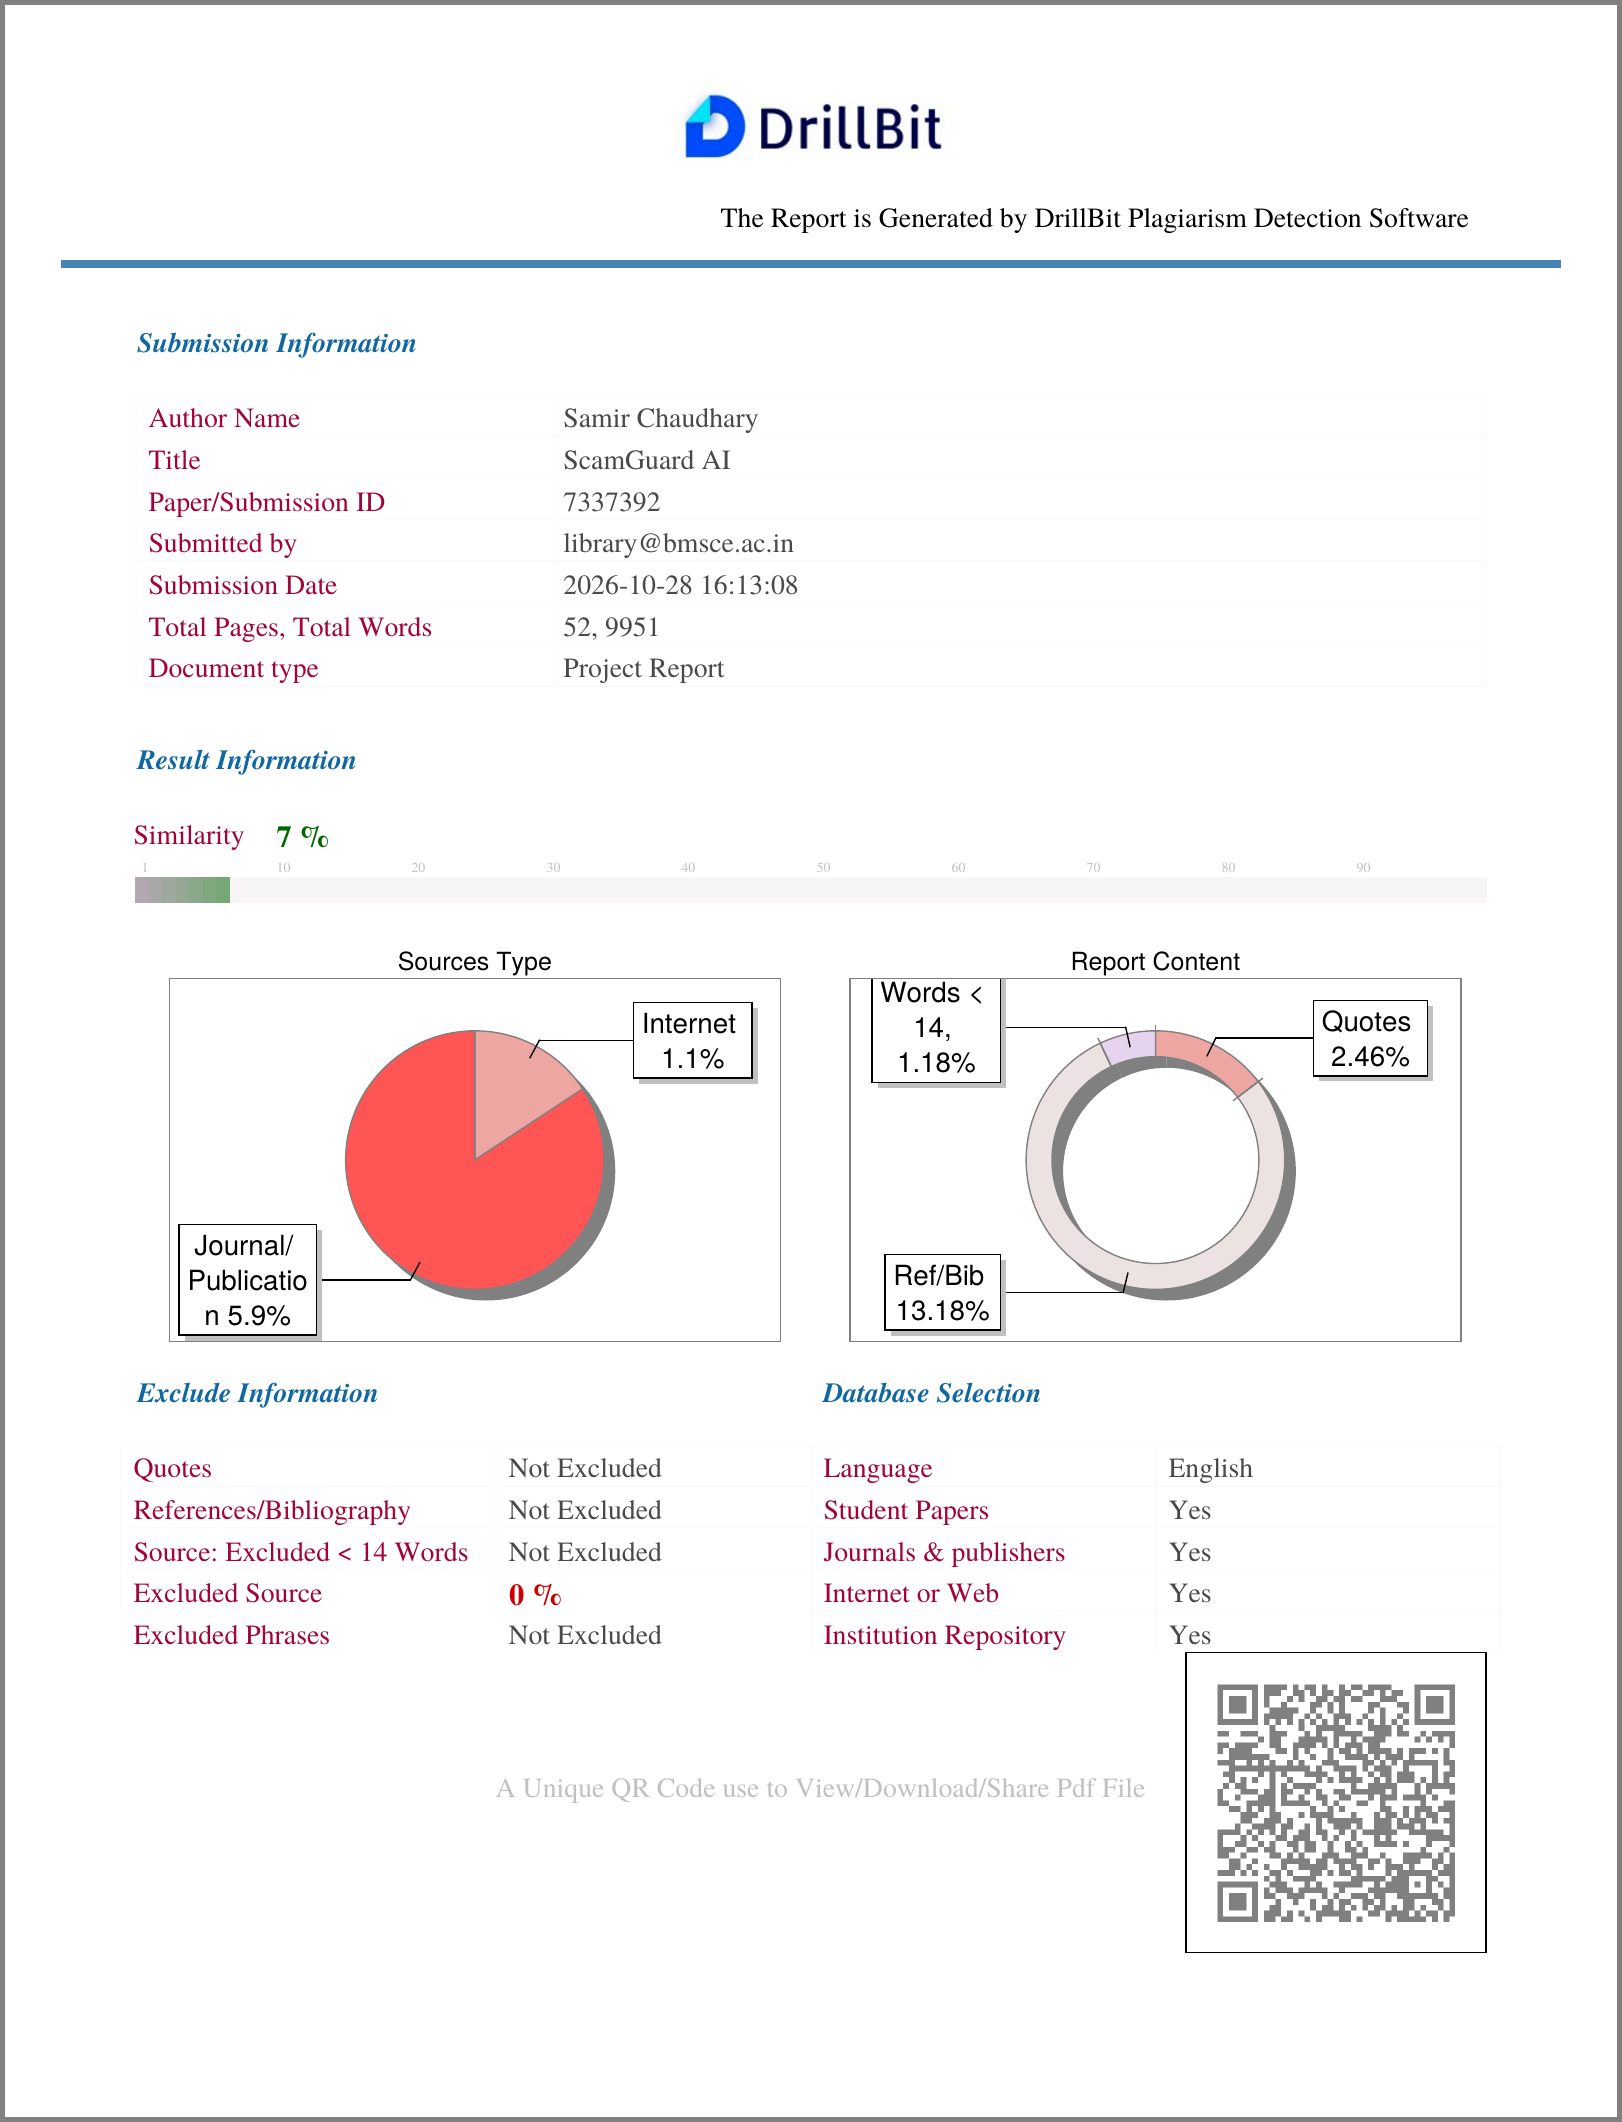
\includegraphics[width=0.92\linewidth,height=0.86\textheight,keepaspectratio]{dbimg/sim-1_c.png}
\end{center}
\clearpage
\begin{center}
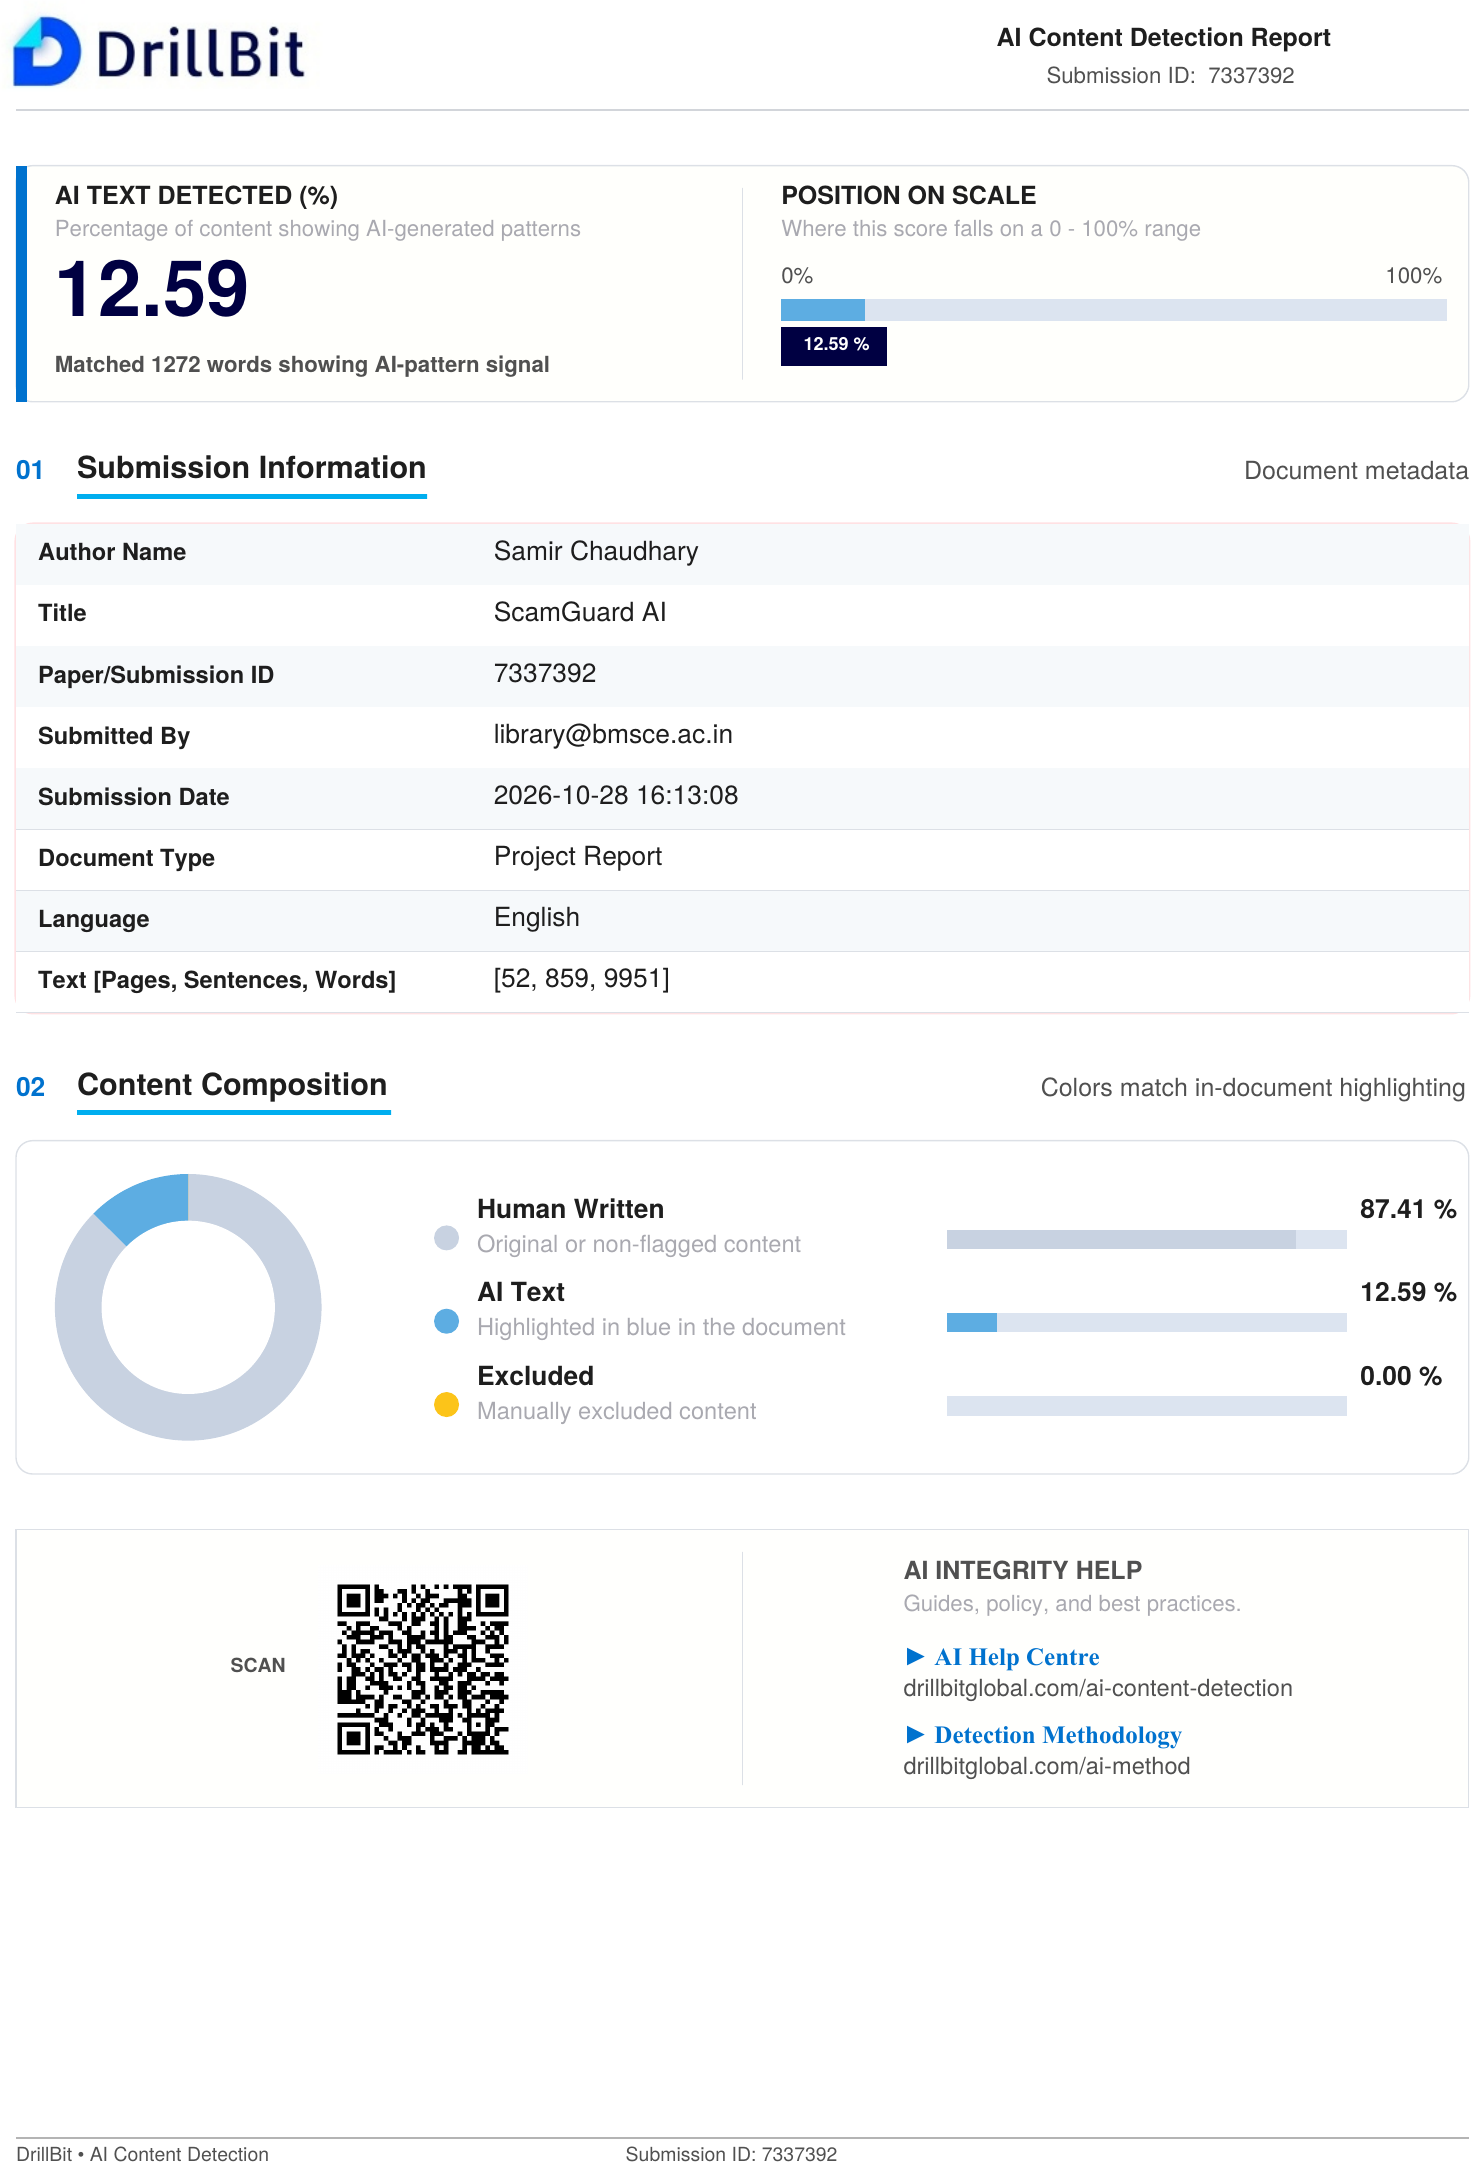
\includegraphics[width=0.92\linewidth,height=0.92\textheight,keepaspectratio]{dbimg/ai-01_c.png}
\end{center}
